\chapter{Introducción}
\section{Objetivo y alcance}
En este documento se detalla el diseño de pruebas para un sistema de gestión de carreras populares.
El sistema permite a los usuarios inscribirse en carreras populares, así como a los organizadores de
las mismas gestionar las inscripciones y la información de las carreras.

El objetivoes diseñar las pruebas necesarias para garantizar que el sistema funciona correctamente.
Para ello, se han identificado las clases de equivalencia y se han diseñado las situaciones y casos
de prueba necesarios para cubrirlas.

Una vez diseñado el conjunto de pruebas, teniendo en cuenta todas las situaciones y valores límite que se
consideran relevantes, se procede a su ejecución y validación, con un posterior reporte ejecutivo que
detallará los resultados obtenidos.

Debido a la complejidad del sistema, el diseño ha de ser robusto, contando con una base de datos donde
se almacenen todos los casos de prueba necesarios para garantizar la cobertura de todas las situaciones
y valores límite.

\section{Descripción del sistema}
\begin{minipage}{\linewidth}
	\centering
	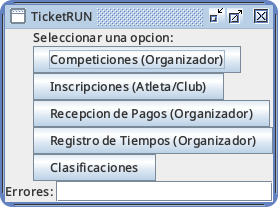
\includegraphics[width=0.4\textwidth]{menu.png}
	\captionof{figure}{Menu principal de la aplicación}
\end{minipage}

El sistema permite tanto a usuarios como a organizadores de carreras populares gestionar la información
relativa a las carreras y las inscripciones en las mismas. Los usuarios pueden inscribirse en las carreras
disponibles, mientras que los organizadores pueden gestionar las inscripciones y la información de las
carreras.

El sistema cuenta con una base de datos donde se almacena toda la información relativa a las carreras y
las inscripciones. Además, cuenta con una interfaz gráfica que permite a los usuarios y organizadores
interactuar con el sistema.
